% 为了方便修改,我们可以先定义一个统一的高度变量
\newlength{\myfigheight}
\setlength{\myfigheight}{7.01cm} % 在这里统一调整三张图的高度

\begin{figure*}[t]
    \centering
    
    % --- 子图 (a) ---
    \begin{subfigure}{\widthof{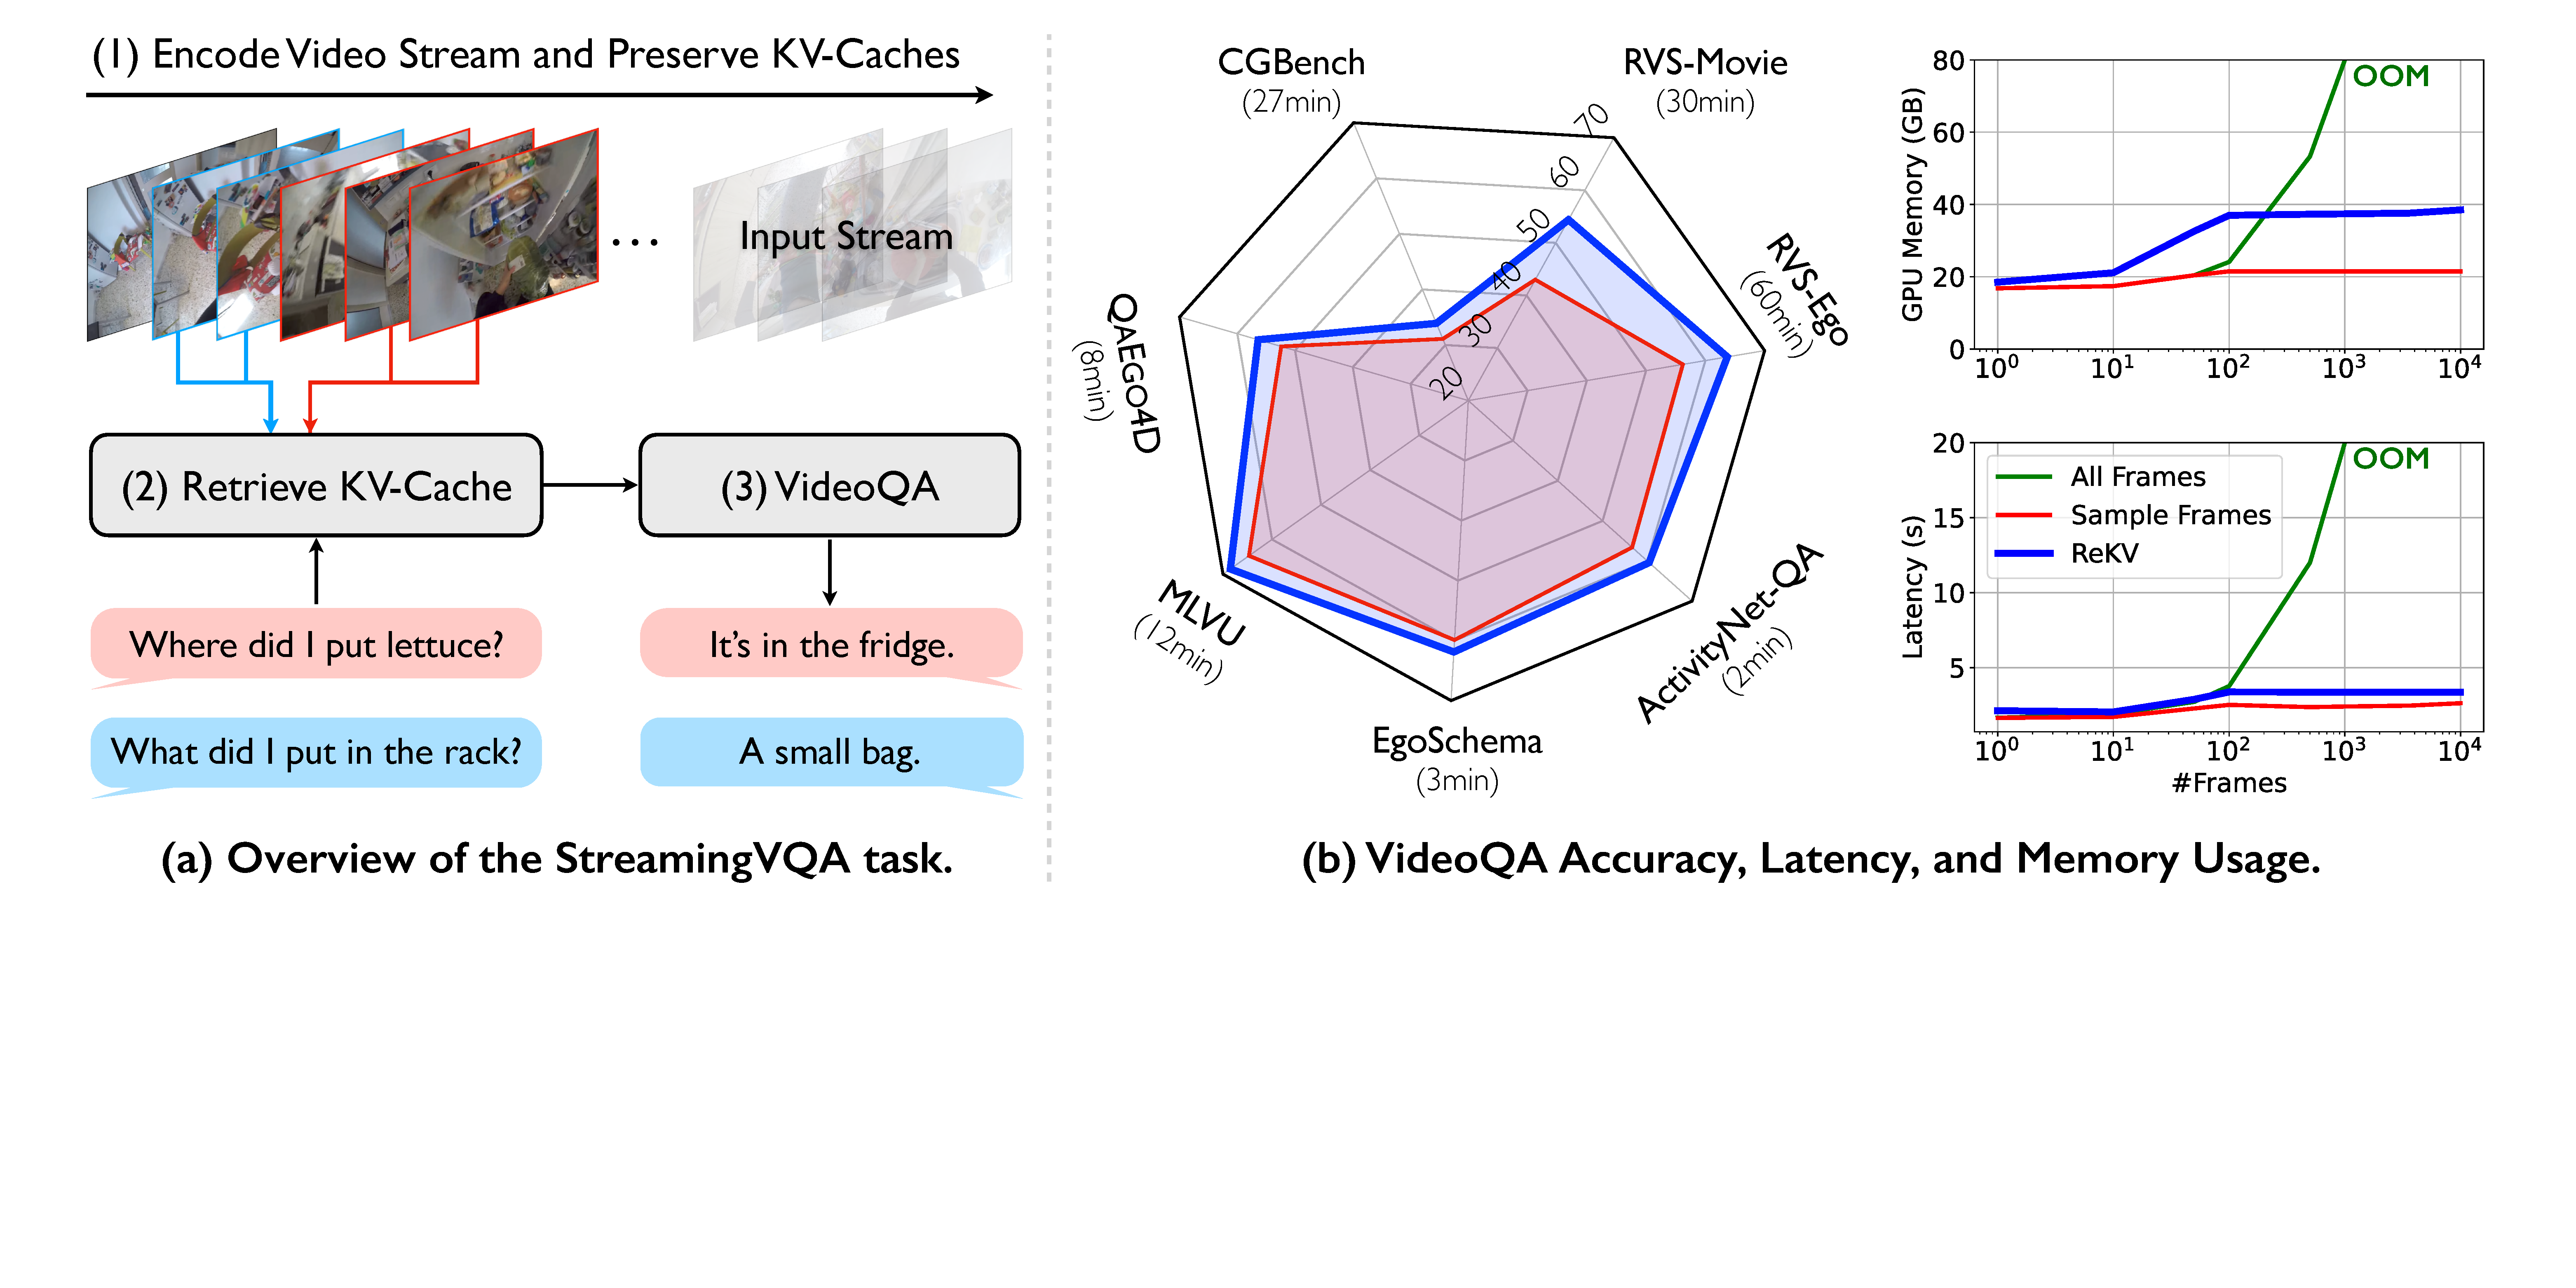
\includegraphics[height=\myfigheight, trim={0 0 415pt 0}, clip]{figures/teaser.pdf}}}
        \centering
        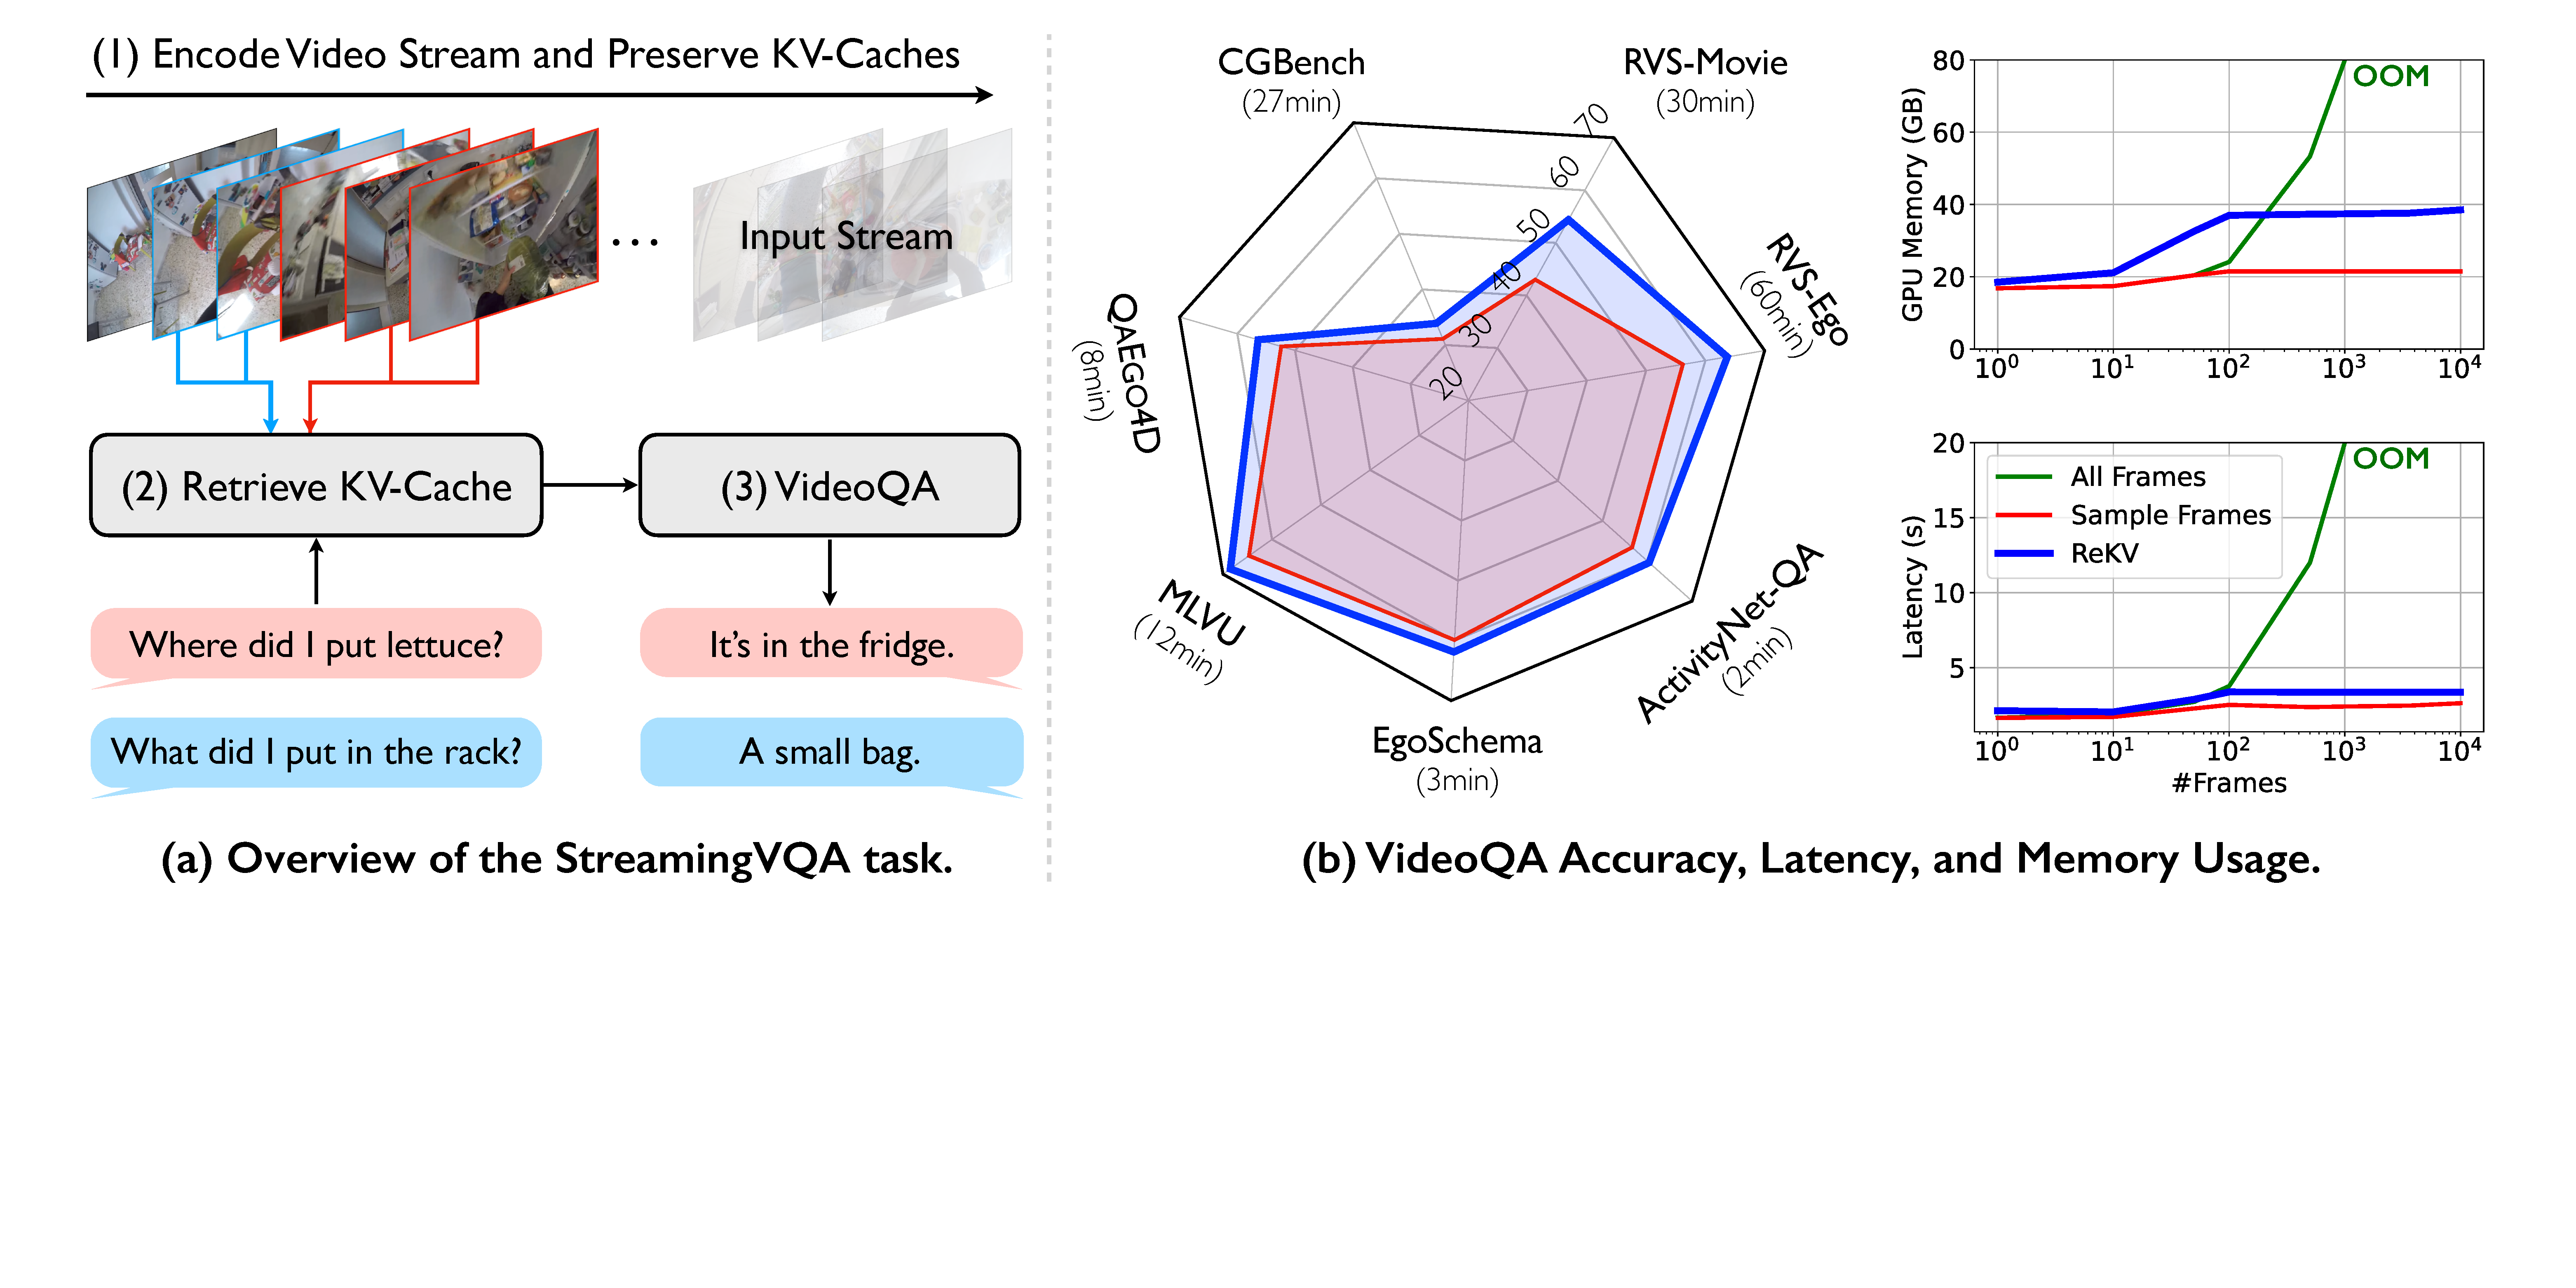
\includegraphics[height=\myfigheight, trim={0 0 415pt 0}, clip]{figures/teaser.pdf}
        \caption{\hermes Framework}
        \label{fig:teaser_a}
    \end{subfigure}
    % --- 子图 (b) ---
    \begin{subfigure}{\widthof{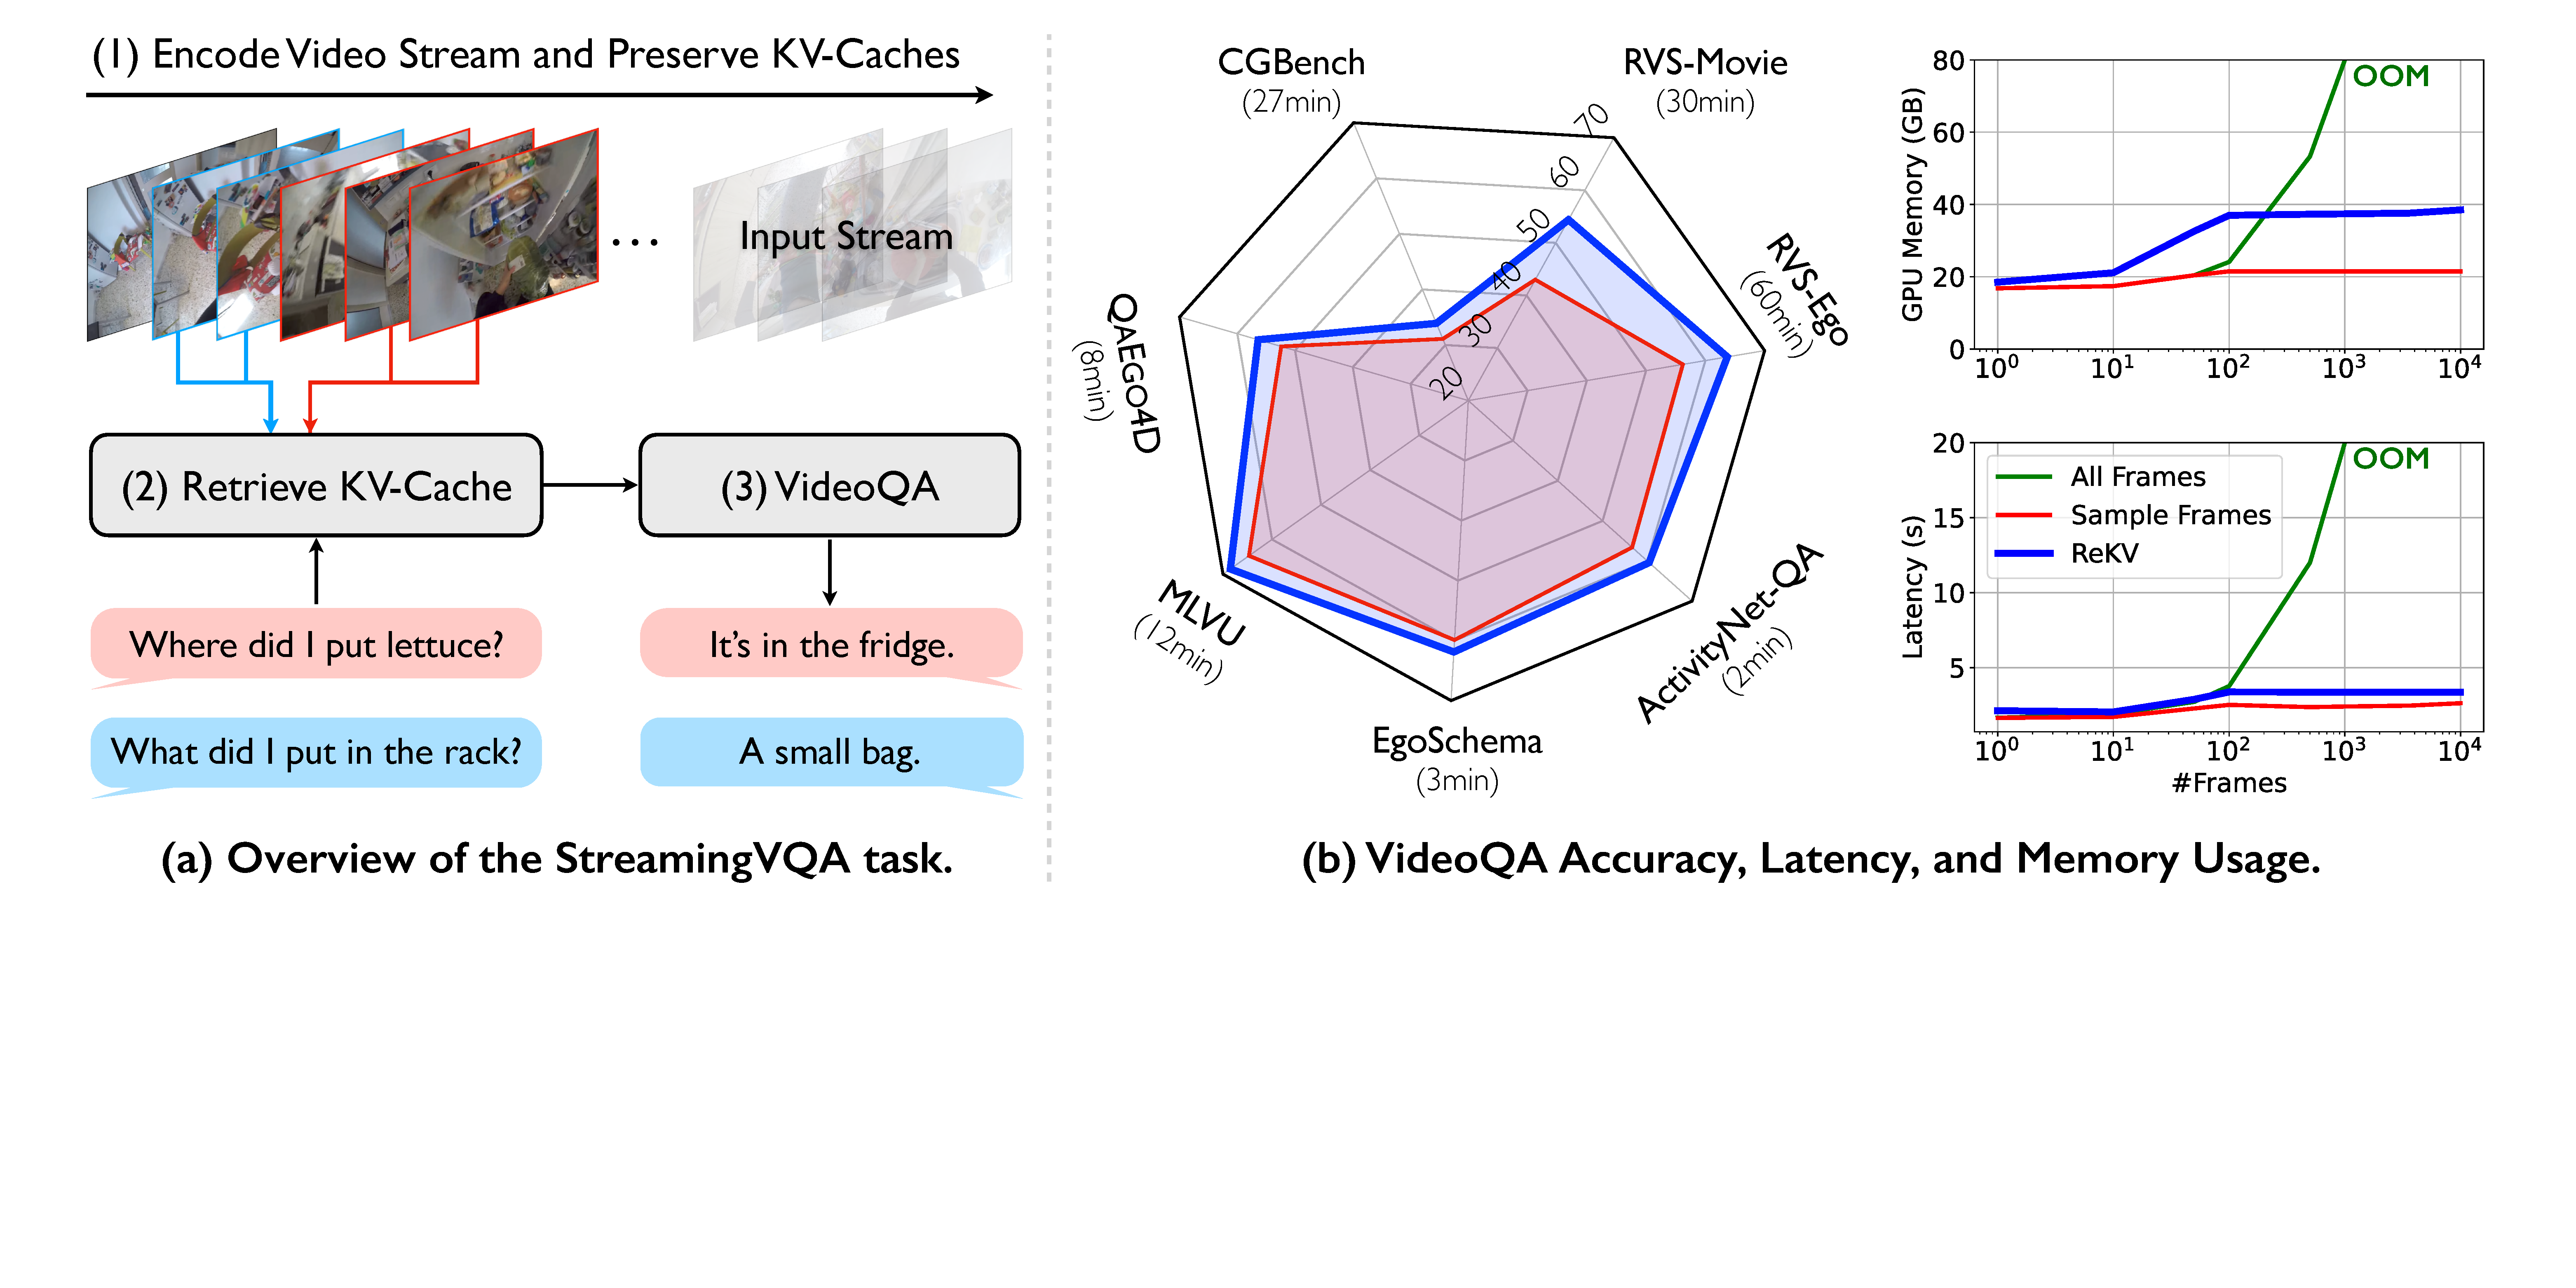
\includegraphics[height=\myfigheight, trim={365pt 0 251pt 0}, clip]{figures/teaser.pdf}}}
        \centering
        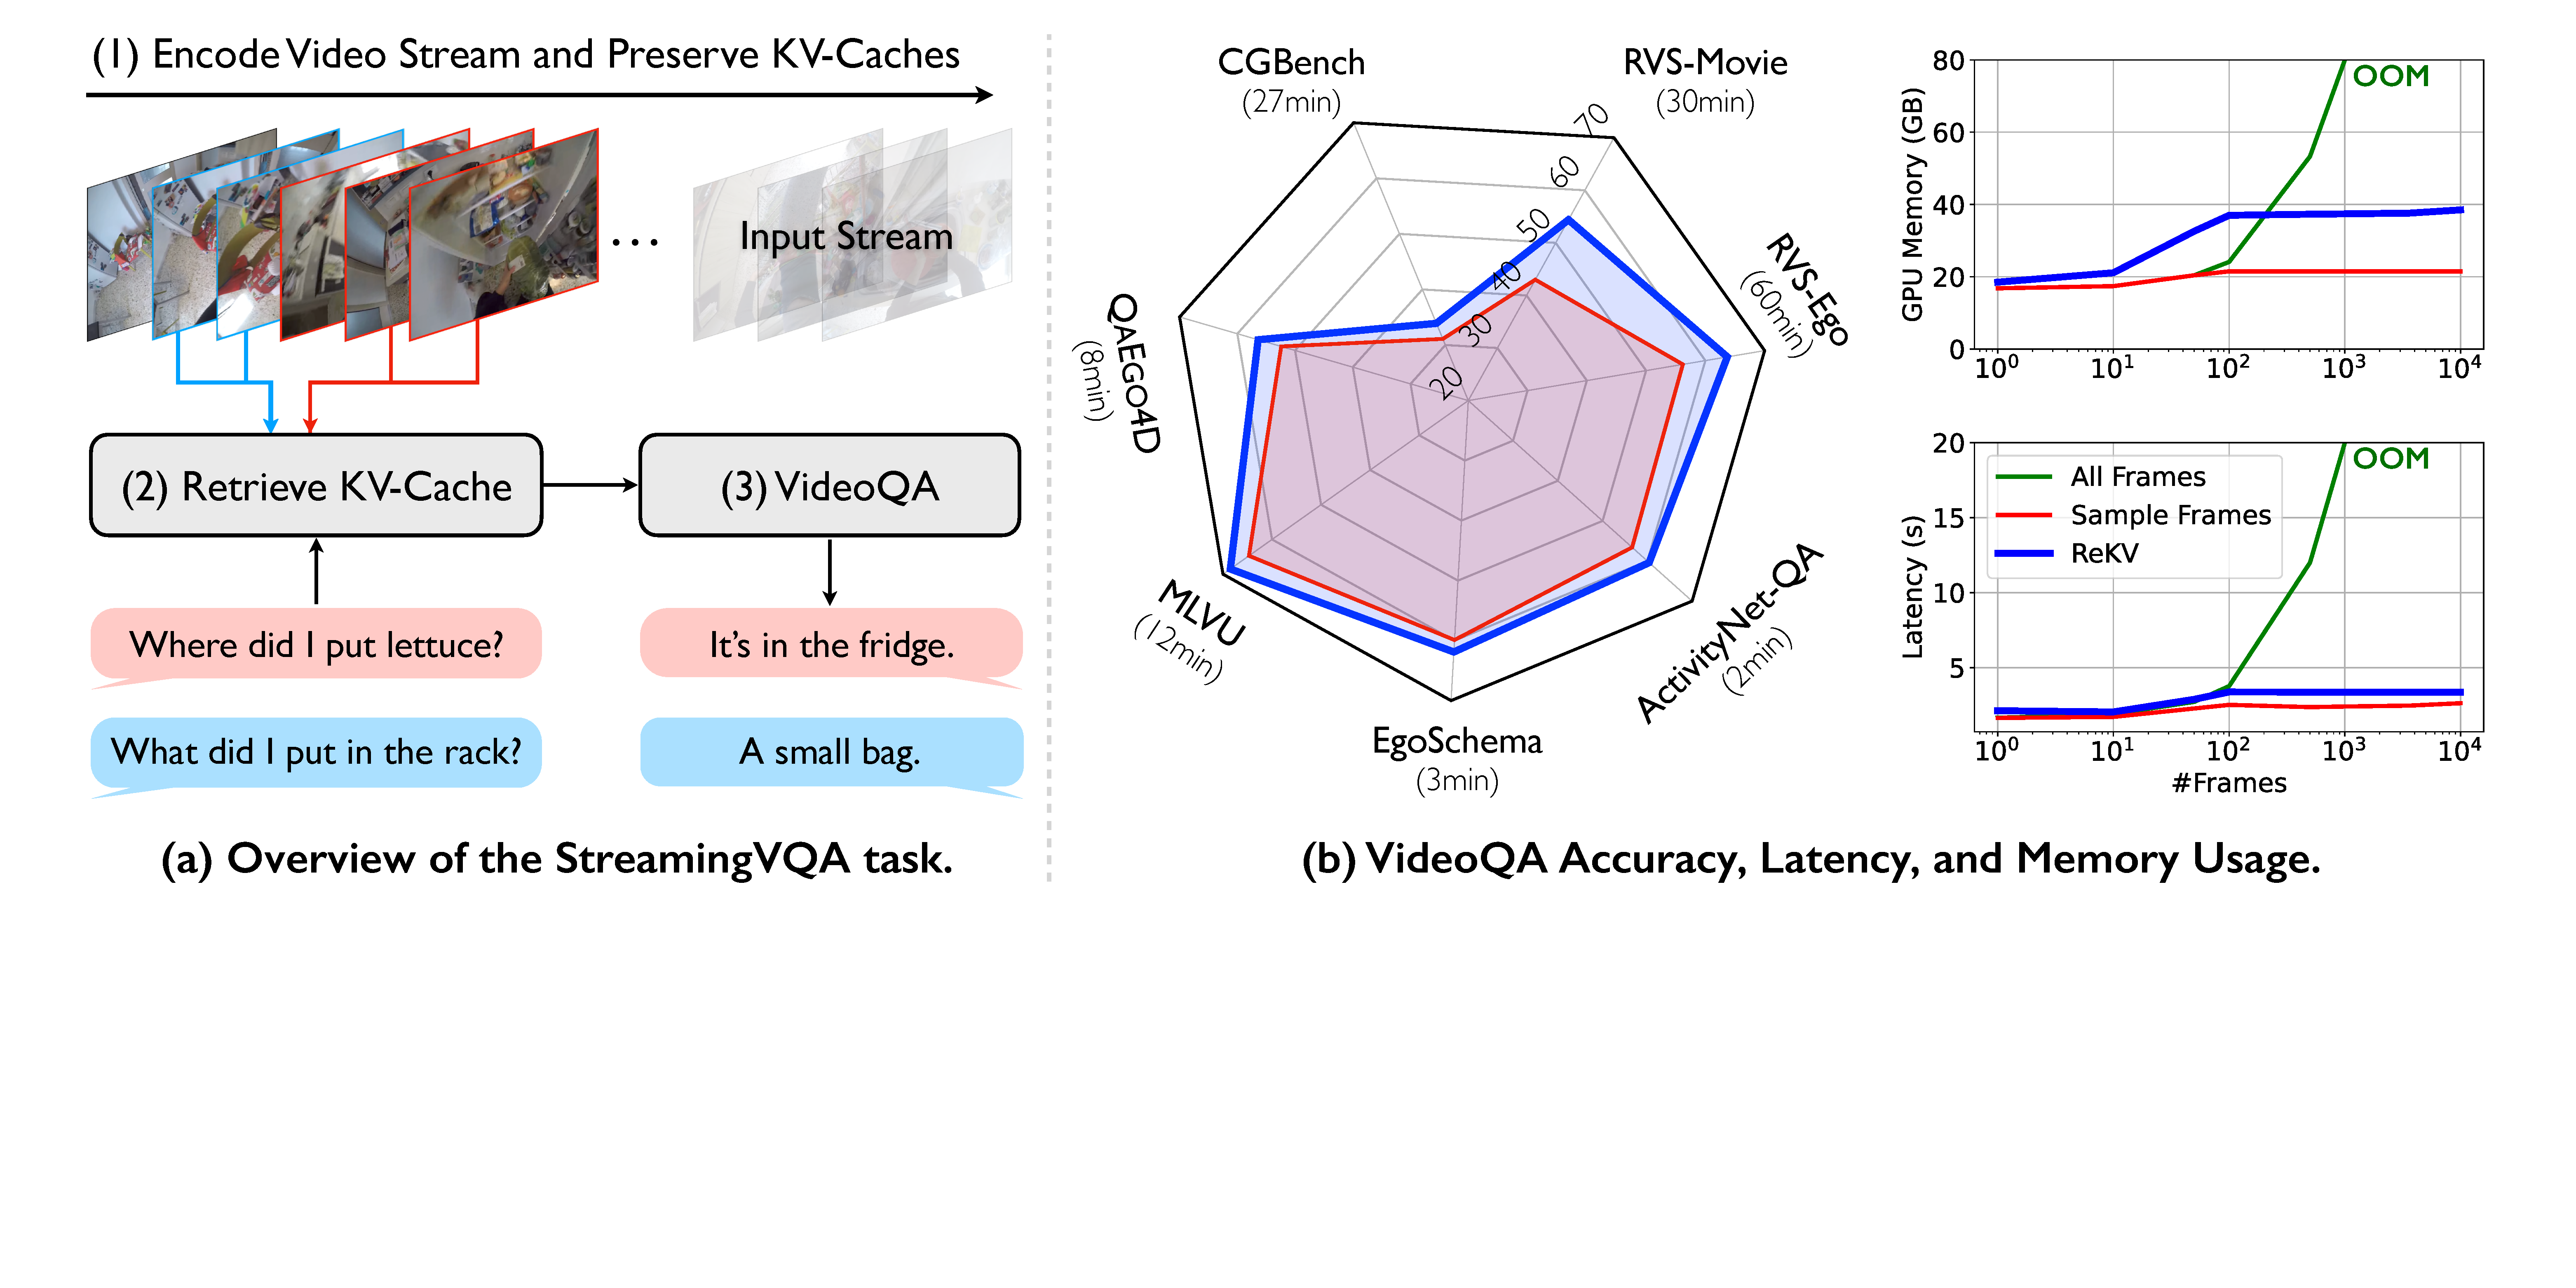
\includegraphics[height=\myfigheight, trim={365pt 0 251pt 0}, clip]{figures/teaser.pdf}
        \caption{Attention Analysis}
        \label{fig:teaser_b}
    \end{subfigure}
    % --- 子图 (c) ---
    \begin{subfigure}{\widthof{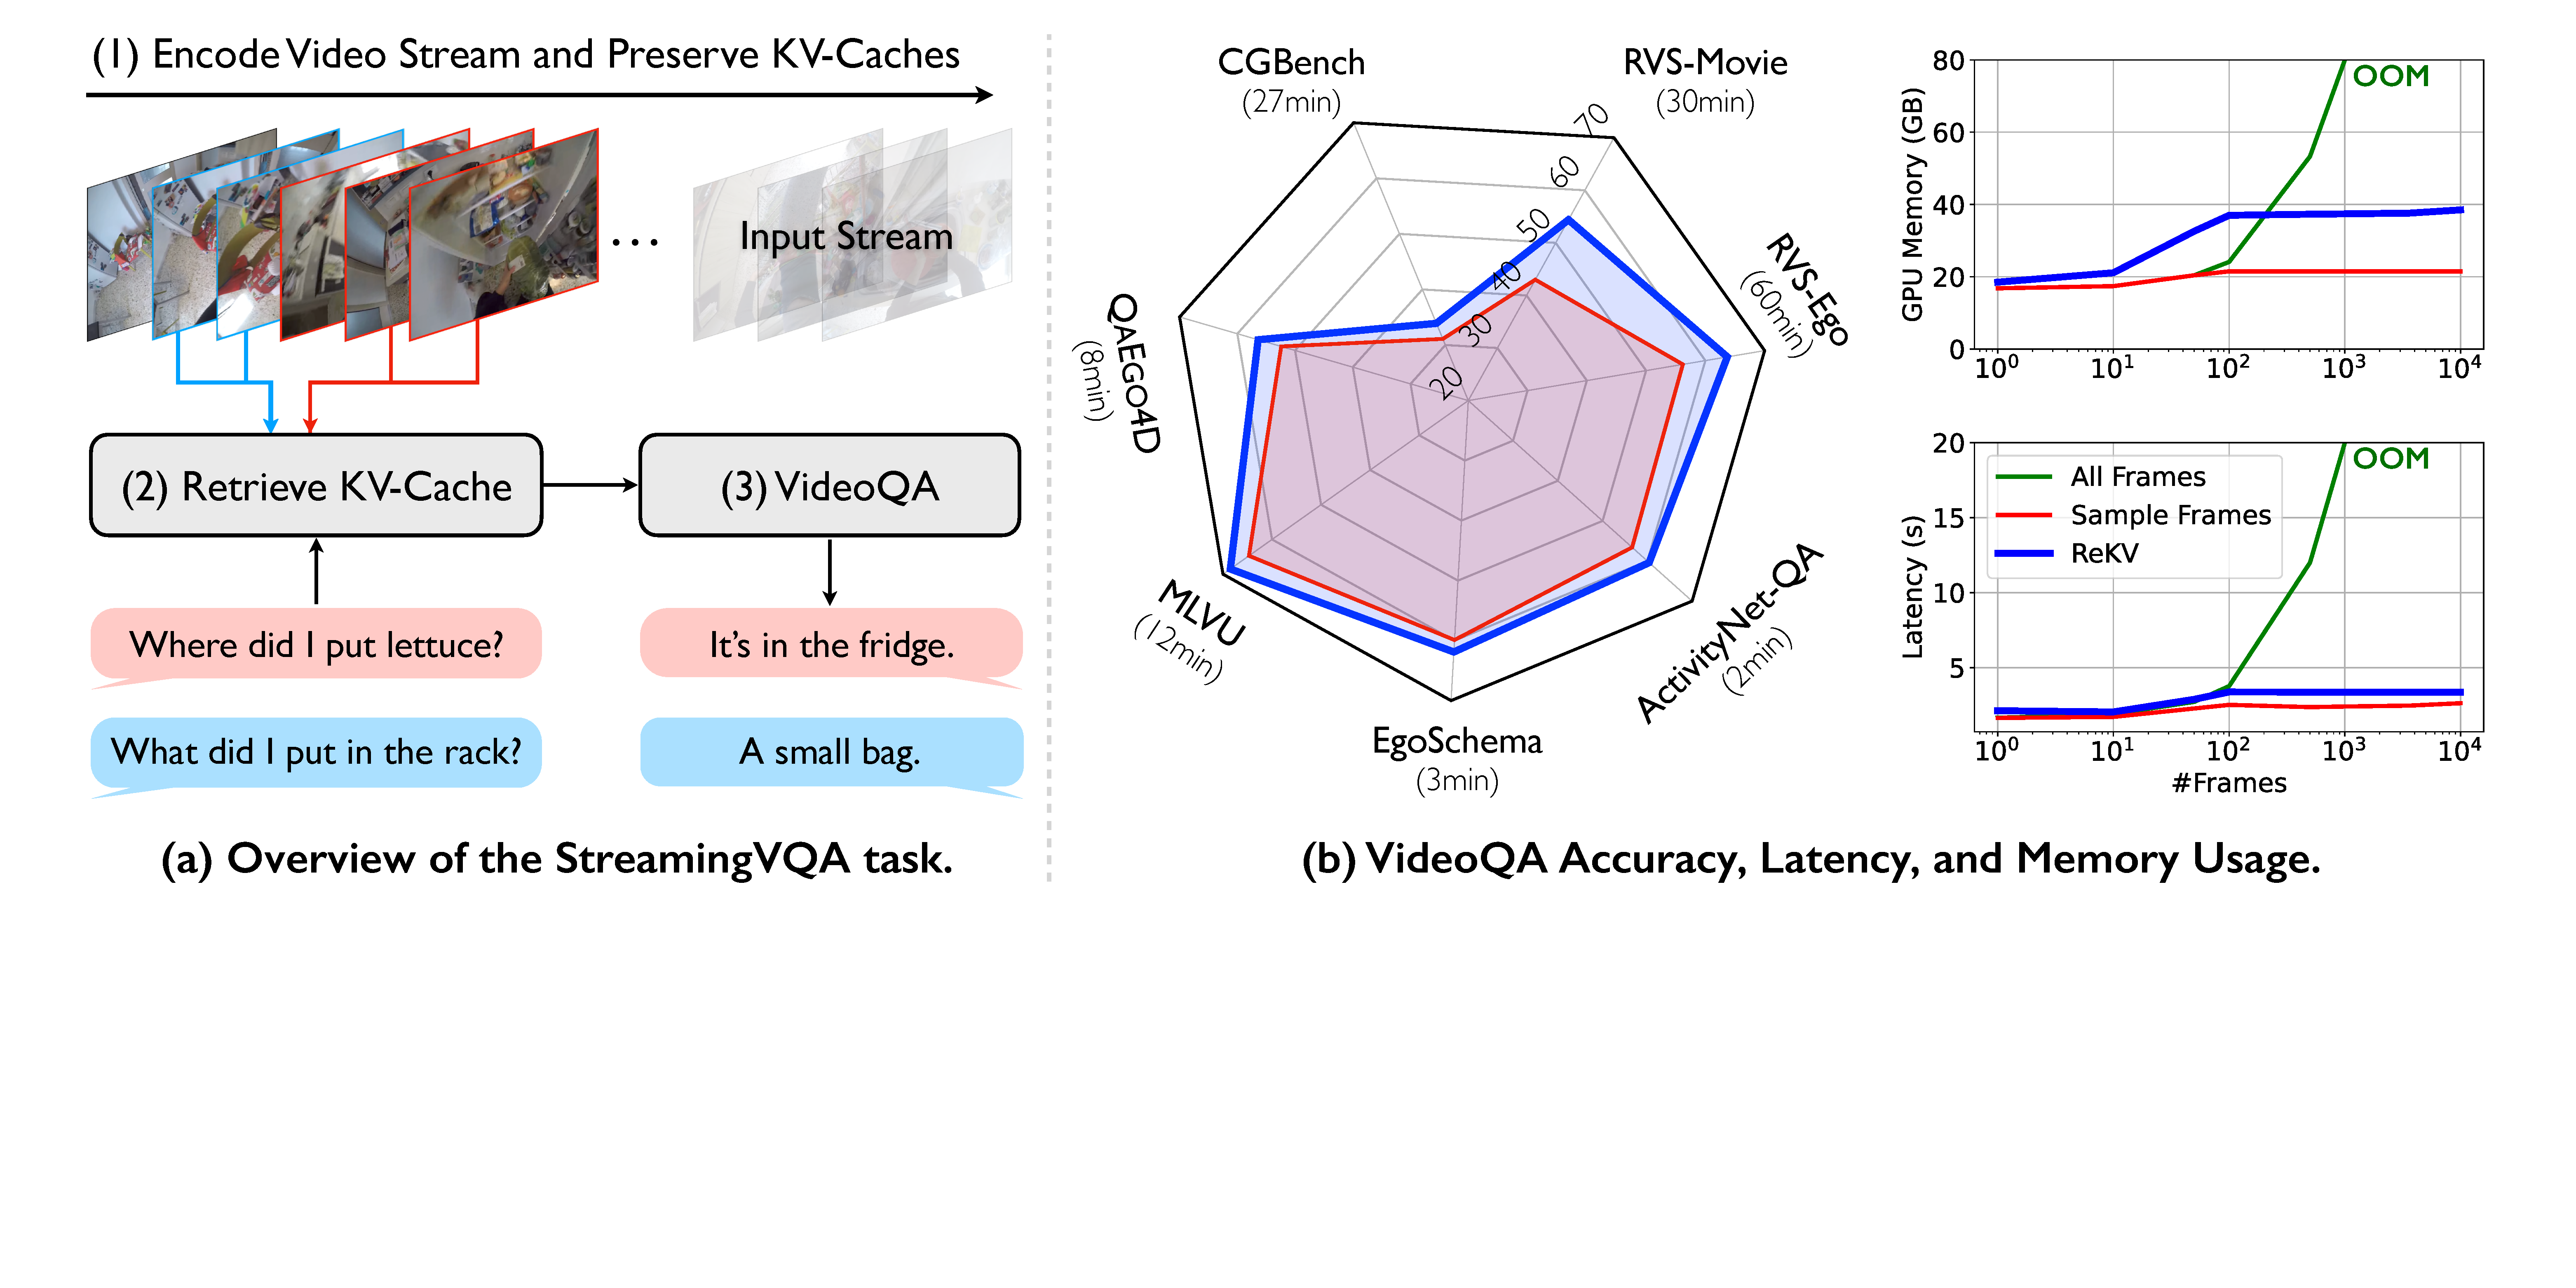
\includegraphics[height=\myfigheight, trim={529pt 0 0 0}, clip]{figures/teaser.pdf}}}
        \centering
        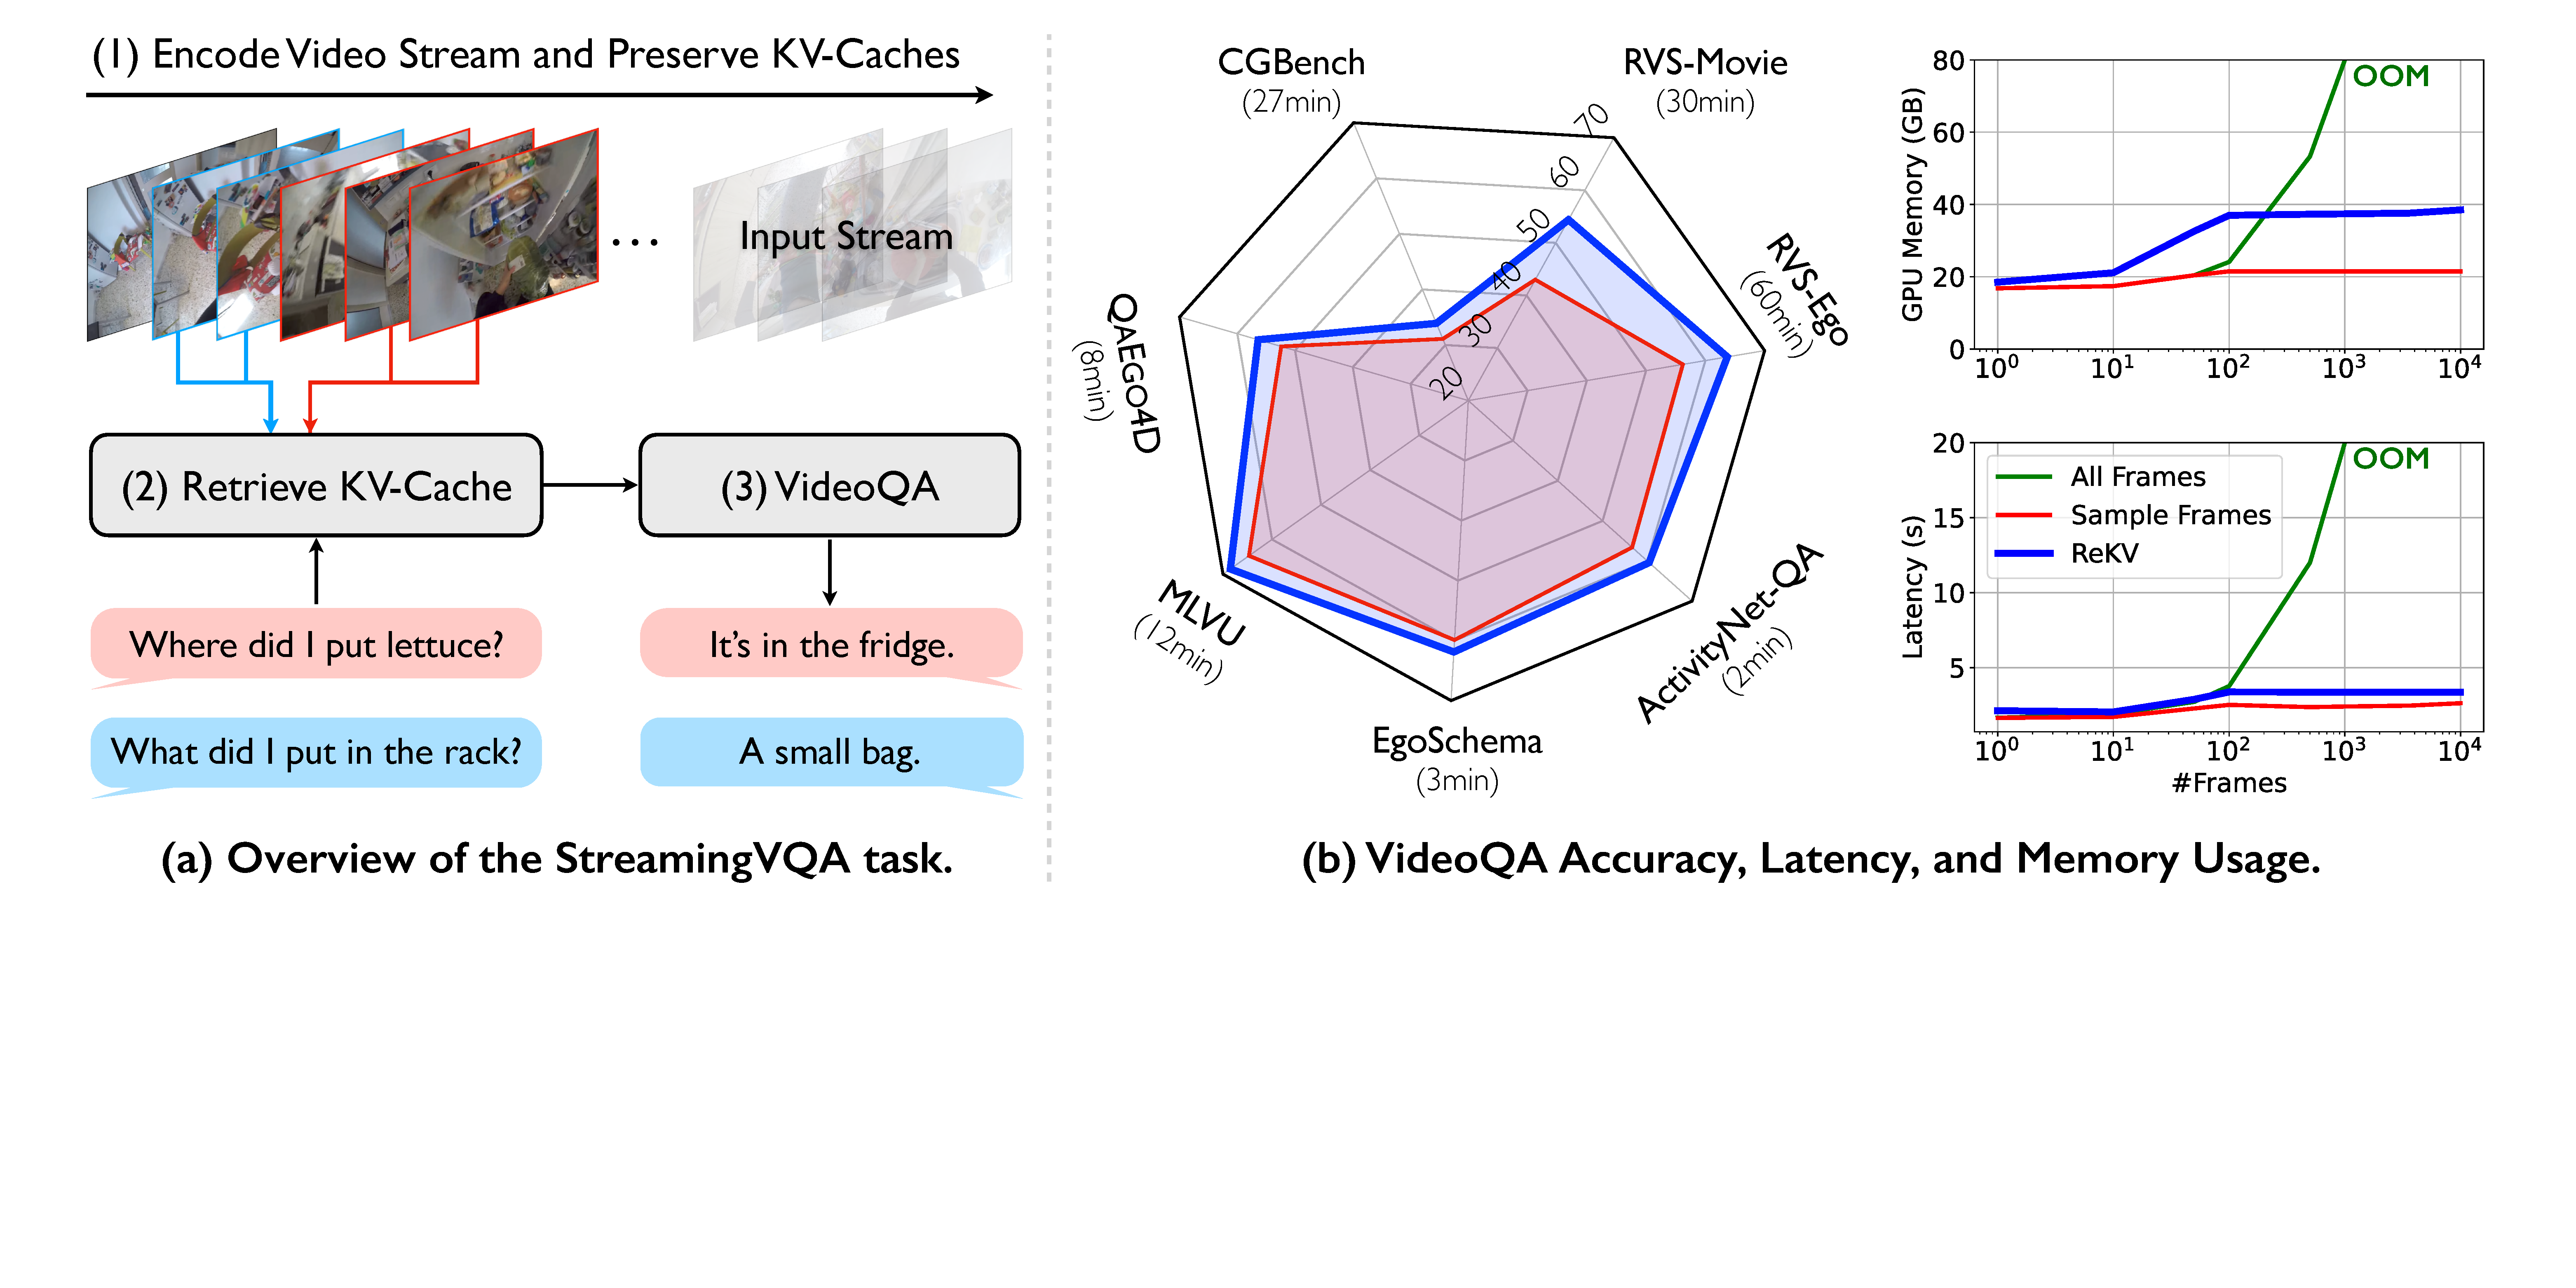
\includegraphics[height=\myfigheight, trim={529pt 0 0 0}, clip]{figures/teaser.pdf}
        \caption{Efficiency Test}
        \label{fig:teaser_c}
    \end{subfigure}
    \caption{\textbf{Left}: \hermes is a training-free approach for efficient streaming video understanding, enabling stable inference by reusing KV cache and performing hierarchical management of video tokens stored in KV cache. \textbf{Middle}: \hermes is based on a mechanistic investigation of the layer-wise attention preferences over hierarchical video information. \textbf{Right}: We evaluate \llava on a single A800 GPU (80 GB). As input frames increase, \hermes consistently maintains extremely low latency (TTFT < 30 ms) and stable GPU memory consumption, exhibiting no risk of OOM errors and requiring no auxiliary external computational resources.}
\end{figure*}


